% LaTeX file for resume 
% This file uses the resume document class (res.cls)

\documentclass{res} 
\usepackage{tikz}
\usepackage[margin=0.7in]{geometry}
\usetikzlibrary{trees}
%\usepackage{helvetica} % uses helvetica postscript font (download helvetica.sty)
%\usepackage{newcent}   % uses new century schoolbook postscript font 
\setlength{\textheight}{12in} % increase text height to fit on 1-page 
\addtolength{\topmargin}{-.275in}
\addtolength{\textwidth}{.75in}
\usepackage{fancyhdr}
\pagestyle{fancy}
\newsectionwidth{-0.35in}

\begin{document} 

\rhead{170 East $6^{th}$ Street \#928 \\
Claremont, CA 91711}

\lhead{Ziv.Epstein@pomona.edu \\
Zepstein.com; 303.993.9411}

   \vspace{0.4in}
\name{\hspace{0in} Ziv G. Epstein}     % the \\[12pt] adds a blank
				        % line after name                   
\begin{resume}
	     \vspace{-0.3in}	
	     
	\begin{center}
	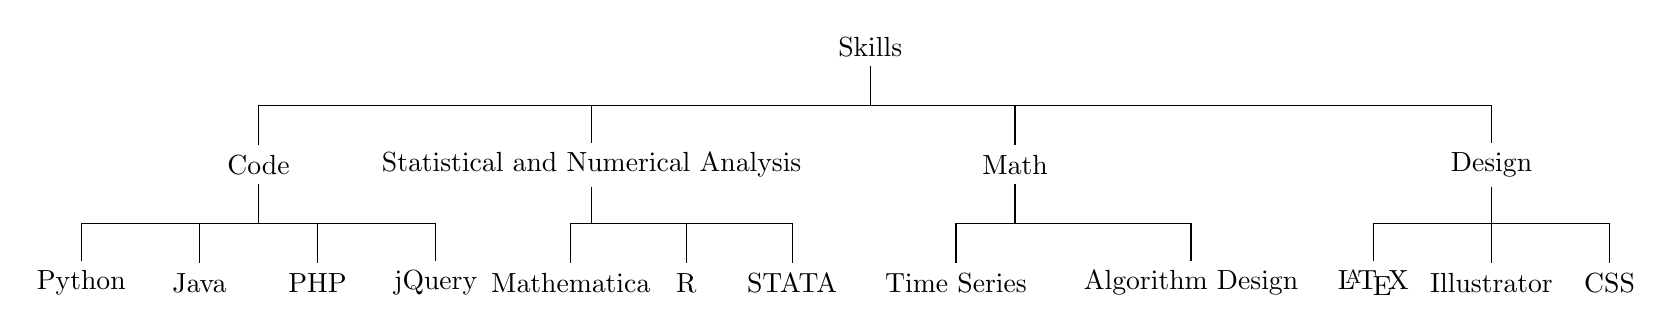
\begin{tikzpicture}[edge from parent fork down,
	edge from parent/.style={black,thin,draw}]
	\node at (-4,4)[left=5cm] {Skills }
	child {node[left=5cm] {Code}
		child {node {Python}}
		child {node {Java}}
		child {node {PHP}}
		child {node {jQuery}}
		}
	child {node[left=0cm] {Statistical and Numerical Analysis}
		child {node[right=.1cm] {Mathematica}}
		child {node[right=.95cm] {R}}
		child {node [right=.35cm]{STATA}}}
	child {node [right=.55cm] {Math}
			child {node {Time Series}}
			child {node [right=.0cm]{Algorithm Design}}}
	child {node[right=5cm] {Design}
		child {node {\LaTeX}}
		child {node {Illustrator}}
		child {node {CSS}}
	};

	\end{tikzpicture}
		\end{center}
			     \vspace{-0.35in}	
\noindent\rule{20cm}{0.4pt}
     \vspace{.1in}	
\hspace{3.2in}{\bf EDUCATION}
   \vspace{-0.3in}	
   \begin{tabbing}
   \hspace{2.3in}\= \hspace{2.6in}\= \kill % set up two tab positions
    {\bf Pomona College}, Claremont, CA  \>     \>~~~~~~~~~~~~~~~~~~~~~~~~~~~~~~~Expected May 2017
   \end{tabbing}\vspace{-20pt}      % suppress blank line after tabbing    
Computer Science and Mathematics, GPA 3.90/4.0



\hspace{3.2in}{\bf EXPERIENCE}

   \vspace{-0.3in}	
     \begin{tabbing}
     	\hspace{2.3in}\= \hspace{2.6in}\= \kill % set up two tab positions
     	{\bf Massachusetts Institute of Technology}, Cambridge, MA    \>     \>~~~~~~~~~~~~~~~~~~~~~~~~~~~~~~June 2015 - Present
     \end{tabbing}\vspace{-20pt}      % suppress blank line after tabbing
     Research Assistant at Laboratory for Social Machines in Media Lab\\
     \vspace{-0.15in}	
     \begin{itemize}
     	\item Design web scraper with visualization interface to navigate, quantify, aggregate and thus understand online\\ journalism. Internship affiliated with the MIT Summer Research Program.
     \end{itemize}
     \vspace{-0.2in}	
   \begin{tabbing}
   \hspace{2.3in}\= \hspace{2.6in}\= \kill % set up two tab positions
    {\bf Yale University}, New Haven, CT    \>     \>~~~~~~~~~~~~~~~~~~~~~~~~~~October 2012 - Present
   \end{tabbing}\vspace{-20pt}      % suppress blank line after tabbing
   Data Science Researcher at Human Cooperation Lab\\
     \vspace{-0.15in}	
    \begin{itemize}
\item Design experiments and computational models, collect/analyze data using Machine Learning techniques and\\ write papers to study and quantify human cooperation within an interdisciplinary environment. Funded by\\ Pomona College Summer Internship Grant.
\end{itemize}
     \vspace{-0.2in}	
   \begin{tabbing}
   \hspace{2.3in}\= \hspace{2.6in}\= \kill % set up two tab positions
    {\bf Harvard University}, Cambridge, MA \>   \>~~~~~~~~~~~~~~~~~~~~~~~June 2012 - October 2012             
   \end{tabbing}\vspace{-20pt}
    Intern at Moral Cognition Lab\\
    \vspace{-0.15in}	
\begin{itemize}
\item Designed experiments, ran in-lab studies and learned literature for moral psychology as only high-school \\student in upper division summer  internship program. \end{itemize}
  
 
 \vspace{0.0in}   
\hspace{2.7in}{\bf EXTRACURRICULAR ACTIVITIES}
 \vspace{-0.2in}	         
\begin{tabbing}%
  
   \hspace{2.3in}\= \hspace{2.6in}\= \kill % set up two tab positions          
   {\bf Liason to Pomona Math Department}, Claremont, CA \> \>~~~~~~~~~~~~~~~~~~~~~~~~~~~~~~~June 2014 - Present
   \end{tabbing}\vspace{-21pt}
    Plan department activies and serve as intermediary between Pomona math students and professors.
    \vspace{-0.175in}
   \begin{tabbing}%
   \hspace{2.3in}\= \hspace{2.6in}\= \kill % set up two tab positions
   {\bf KSPC 88.7 FM}, Claremont, CA \> \>~~~~~~~~~~~~~~~~~~~~~~~~~~~~~~~May 2014 - Present
   \end{tabbing}\vspace{-21pt}
    Broadcast weekly underground radio show as volunteer DJ at local college radio station.
    \vspace{-0.175in} 
   \begin{tabbing}%
    \hspace{2.3in}\= \hspace{2.6in}\= \kill % set up two tab positions          
   {\bf Cross Country and Track \& Field}, Claremont, CA \> \>~~~~~~~~~~~~~~December 2013 - November 2014
   \end{tabbing}\vspace{-21pt}
   	Competing and training as a member of Pomona-Pitzer varsity athletic program.

        

  
\hspace{1.62in}{\bf PRESENTATATIONS, AWARDS AND PUBLICATIONS}
 \vspace{0.1in}	
\begin{itemize}
	 \setlength\itemsep{.1em}
 \item Rand DG, \& {\bf Epstein ZG}. Risking Your Life Without a Second Thought: Intuitive Decision-Making and Extreme Altruism. \textit{PLoS ONE} October 15, 2014. Listed as one of the Top 10 Insights from the Science of a Meaningful Life in 2014 by the Greater Good Science Center at UC Berkeley.
\item First Place in 5C Hackathon Advanced category. Built shortest path finding system for Wikipedia (April 2015)
\item D21 Sponsor Prize winner at the Stanford TreeHacks hackathon. Build online political conflict analysis metric using D21 voting paradigm; available online at www.notthatdifferent.meteor.com (February 2015)
\item Second Place in 5C Hackathon Advanced category. Built Online \LaTeX  \ Distribution system available at \\https://github.com/dmsm/DibTeX (November 2014)
\item Padula WV, Allen RR, {\bf Epstein ZG} \& Nair KV. Determining the cost of obesity and common comorbidities from a commercial claims dataset. Health Economics Workshop, University of Chicago; February 27, 2014.
\item The Jaeger Mathematics Prize (September 2014) 
\item Pomona College Scholar (Fall 2013, 2014 and Spring 2014)
\item 1st Place in Social Science Section of CordenPharma Colorado Science Fair (February 2013)
\item National AP Scholar with Distinction (August 2013)
\item Colorado School of Mines Outstanding High School Junior in Math and Science (May 2012)	
% \item Boulder High Student Ambassador to the Rotary Club (March 2012)
\end{itemize} 
 
\end{resume}
\end{document}